\documentclass[a4paper, 12pt]{article}
\usepackage[T2A,T1]{fontenc}
\usepackage[utf8]{inputenc}
\usepackage[english, russian]{babel}
\usepackage{graphicx}
\usepackage[hcentering, bindingoffset = 10mm, right = 13 mm, left = 13 mm, top=20mm, bottom = 20 mm]{geometry}
\usepackage{multirow}
\usepackage{lipsum}
\usepackage{amsmath, amstext}
\usepackage{siunitx}
\usepackage{subcaption}
\usepackage{wrapfig}
\usepackage{mathrsfs}
\usepackage{adjustbox}
\usepackage{enumerate, indentfirst, float}
\usepackage{capt-of, svg}
\usepackage{icomma}
\usepackage{xcolor}
\usepackage{ctable}
\usepackage{amssymb}
\usepackage[version=4]{mhchem}
\usepackage{expl3}
\usepackage{calc}


\newenvironment{bottompar}{\par\vspace*{\fill}}{\clearpage}
 
\begin{document}
\begin{titlepage}

\newcommand{\HRule}{\rule{\linewidth}{0.5mm}} % Defines a new command for the horizontal lines, change thickness here

\center % Center everything on the page
 
%----------------------------------------------------------------------------------------
%	HEADING SECTIONS
%----------------------------------------------------------------------------------------

\textsc{\LARGE Московский физико-технический институт\\(государственный университет)}\\[1,5cm] % Name of your university/college
\textsc{\Large Департамент молекулярной и биологической физики}\\[2cm] % Major heading such as course name
\textsc{\large Лабораторная работа}\\[0.5cm] % Minor heading such as course title

%----------------------------------------------------------------------------------------
%	TITLE SECTION
%----------------------------------------------------------------------------------------

\HRule
\\[0.4cm]
{ \huge \bfseries Кинетика йодирования ацетона}
\\[0.2cm] % Title of your document
\HRule
\\[1.5cm]


 
%----------------------------------------------------------------------------------------
%	AUTHOR SECTION
%----------------------------------------------------------------------------------------
\begin{minipage}{0.4\textwidth}
	\begin{flushleft}		
	\end{flushleft}
\end{minipage}
~
\begin{minipage}{0.4\textwidth}
	\begin{flushright} \large
		\emph{Авторы:}\\
		Светлана \textsc{Фролова} \\
		6113 группа \\
		Анатолий \textsc{Киселёв} \\
		6113 группа
	\end{flushright}
\end{minipage}


\begin{bottompar}
	\begin{center}
		
\includegraphics[width = 80 mm]{logo.jpg}
	\end{center}
	{\large г. Долгопрудный\\2018 г.}

\end{bottompar}
\vfill % Fill the rest of the page with whitespace

\end{titlepage}

\setcounter{page}{2}

\newpage
\section{Цели работы}
	\begin{enumerate}
	
		\item 
		Убедиться в справедливости закона Бэра, определить коэффициент молярной экстинкции йода;
		\item
		Проверить независимость скорости йодирования от концентрации йода, изучить зависимость скорости реакции от концентрации кислоты и ацетона;
		\item 
		Рассчитать константу скорости реакции.
		 
	
	\end{enumerate}
	
\section{Теоретическая часть}
Реакция йодирования ацетона в кислом водном растворе
\begin{equation}\label{'gen'}
\ce{CH3C(O)CH3 + I2 + H3O^+ + H2O <--> CH3COCH2I + I^- + 2H3O^+}
\end{equation}
протекает в две стадии. В кислой среде ацетон становится протофильным и присоединяет протон иона гидрооксония:
\begin{equation}\label{'1stage'}
\ce{CH3C(O)CH3 + H3O^+ <--> CH3C^{-}OHCH3^+ + H3O^+}
\end{equation}
Водород метильной группы кетоенола приобретает подвижность и соединяется с молекулой воды:
\begin{equation*}
\ce{CH3C^{-}(OH)CH3 + H2O <--> CH3(OH)CH2 + H3O^+}
\end{equation*}
Таким образом, первая стадия реакции представляет собой превращение кетона в енол. На второй стадии реакции енол присоединяет йод:
\begin{equation}\label{'2stage'}
\ce{CH3(OH)CH2 + I2 + H2O -> CH3COCH2I + 2H3O^+ + I-}
\end{equation}
Вторая стадия (\ref{'2stage'}) реакции протекает значительно быстрее первой и прак-тически до конца. Поэтому скорость реакции (\ref{'gen'}) определяется скоростью обра-зования енола в (\ref{'1stage'}) и не зависит от концентрации йода. Скорость расходова-ния ацетона в системе равна скорости расходования йода. Поскольку в процессе реакции происходит увеличение числа ионов гидрооксония, реакция является автокаталитической. Реакция йодирования протекает по первому порядку для двух реагирующих веществ (ацетон и ион гидрооксония), и исходное дифференциальное уравнение для определения константы скорости реакции $k$ может быть записано в виде:
\[-\frac{dA}{dt}=k\cdot A\cdot H,\]
где $A = [\ce{CH3C(O)CH3}], H = [\ce{H3O+}]$ – текущие концентрации ацетона и ионов гидрооксония. Применяя индекс $0$ для обозначения начального момента времени, после интегрирования уравнения получим для $k$ следующее выражение:
\[k=\frac{1}{\tau}\cdot\frac{1}{A_0+H_0}\ln{\left(\frac{A_0(H_0+x)}{H_0(A_0-x}\right)},\]
где $x$ – изменение концентрации йода за время $\tau$. Если начальные концентрации $A_0$ и $H_0$ выбраны существенно большими, чем концентрация йода, то автокаталитичность реакции~(\ref{'gen'}) несущественна, и мы имеем для $k$: 
\begin{equation}
k\approx \frac{x}{\tau}\cdot\frac{1}{A_0\cdot H_0}
\end{equation}


Значение величины $x$ определяется спектрофотометрическим методом по изменению оптической плотности раствора. Применение спектрофотометра для определения концентрации окрашенного реагента (йода, в нашем случае) основано на существовании зависимости между оптической плотностью раствора и концентрацией в нем окрашенного реагента. Для многих веществ (в диапазоне сравнительно небольших концентраций) эта зависимость является линейной, т.е. справедлив закон Бера (1853г.), который может быть записан в виде:
\begin{equation}\label{Ber}
D = \varepsilon_\lambda\cdot d\cdot C,
\end{equation}
где $D$ – оптическая плотность (коэффициент поглощения света) слоя раствора толщиной $d$, а $\ C$ – концентрация в нем окрашенного реагента. Таким образом, для определения концентрации данного реагента в растворе спектрофотометрическим методом, необходимо знать значение молярного коэффициента экстинкции $\lambda$. Возможность определения концентрации йода в исследуемом реакционном растворе обусловлена малостью оптических плотностей всех исходных веществ и продуктов реакции по сравнению с йодом (на используемой длине волны 520 нм).

\newpage
\section{Обработка результатов}
Снимем спектры для растворов с разными концентрациями йода (рисунок \ref{spc}), построим график зависимости оптической плотности $D$ от концентрации \ce{[J2]}.\\

\begin{figure}[h]
	\centering
	\caption{Спектр}\label{spc}
	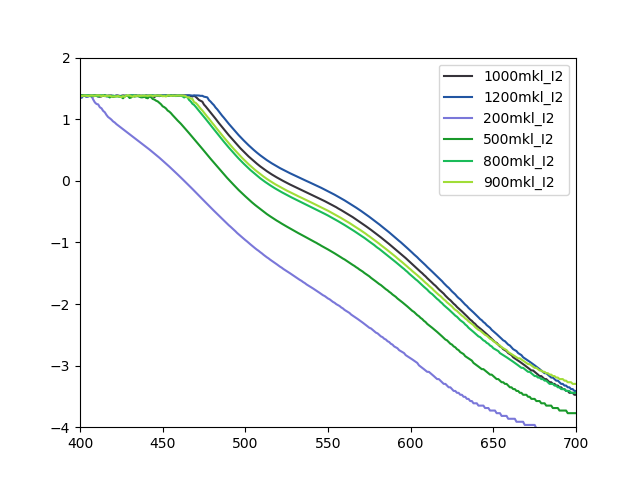
\includegraphics[width=1\textwidth]{Spector.png}
\end{figure}
Отсюда получим зависимость оптической плотности $D$ от объёма добавленного йода на длине волны $\lambda=480\ \text{нм}$. Данные приведены в таблице \ref{kaltabl}.\\ 

\begin{table}[h!]
	\centering
	\caption{}\label{kaltabl}

	\begin{tabular}{|c|c|}

\hline 
$V_{\ce{J2}},\ \text{мкл}$ & D \\ 
\hline 
$200\pm 10 $& $0,632\pm 0,001$ \\ 
\hline 
$500\pm 10 $& $1,385\pm 0,001$ \\ 
\hline 
$800\pm 10 $& $2,386\pm 0,001$ \\ 
\hline 
$900\pm 10 $& $2,557\pm 0,001$\\ 
\hline 
$1000\pm 10 $& $2,928\pm 0,001$ \\ 
\hline 
$1200\pm 20 $& $3,507\pm 0,001$ \\ 
\hline 

	\end{tabular} 
\end{table}

\newpage
Построим калибровочный график (рисунок \ref{kal}):\\

\begin{figure}[h]
	\centering
	\caption{}\label{kal}
	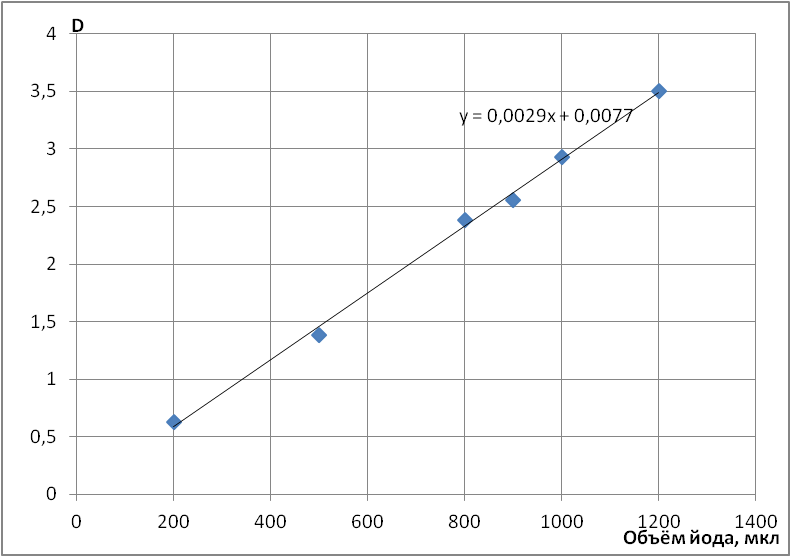
\includegraphics[width=0.6\textwidth]{image001.png}
\end{figure}

Получили линейную зависимость, что подтверждает закон Бера (\ref{Ber}).
Найдём коэффициент экстинкции из закона Бера (\ref{Ber}):
\[\varepsilon_\lambda=(340\pm 30)\textstyle \frac{\text{л}}{\text{моль}\cdot\text{см}}\]

В таблице \ref{bigtable} приведенs данные углового коэффициента $y$ графиков, построенных в координатах $D=f(t)$ при изменении концентрации одного из реагентов и фиксированных других, т.е. $y_i=\frac{d D_i}{d t}\sim \frac{d C_i}{d t}$ .\\ 

\begin{table}[h!]
\centering
\caption{}\label{bigtable}
\begin{tabular}{|c|c|c|c|}
\hline
\multicolumn{4}{|c|}{\ce{J2}}             \\ \hline
$V,\ \mu l$    & $y, c^{-1}$       & $\ln{V}$     & $\ln{y}$     \\ \hline
$400\pm 10$  & $-0,029\pm 10^{-5}$  & $5,991465\pm 0,03$ & $-3,54046 $\\ \hline
$640\pm 10$  & $-0,029\pm 10^{-5}$  & $6,461468\pm 0,02 $&$ -3,54046 $\\ \hline
$800\pm 10$  & $-0,026\pm 10^{-5}$  & $6,684612\pm 0.02 $&$ -3,64966 $\\ \hline
$1200\pm 20$ & $-0,03\pm 10^{-5}$   & $7,090077\pm 0,02 $&$ -3,50656 $\\ \hline
\multicolumn{4}{|c|}{\ce{HCl}}            \\ \hline
$V,\ \mu l$    & $y, c^{-1}$       & $\ln{V}$     & $\ln{y}$     \\ \hline
$300\pm 10$  & $-0,0013\pm 10^{-5}$ & $5,703782\pm 0,03 $&$ -6,64539 $\\ \hline
$600\pm 10$  & $-0,0026\pm 10^{-5}$ & $6,39693\pm 0,02 $ &$ -5,95224$\\ \hline
$900\pm 10$  & $-0,0036\pm 10^{-5}$ & $6,802395 \pm 0,02$&$ -5,62682 $\\ \hline
$1200\pm 20$ & $-0,0052\pm 10^{-5}$ & $7,090077 \pm 0,02$&$ -5,2591  $\\ \hline
\multicolumn{4}{|c|}{\ce{C3H6O}}        \\ \hline
$V,\ \mu l$    & $y, c^{-1}$       & $\ln{V}$     & $\ln{y}$     \\ \hline
$300\pm 10$  & $-0,0012\pm 10^{-5}$ & $5,703782\pm 0,03 $&$ -6,72543 $\\ \hline
$600\pm 10$  & $-0,0021\pm 10^{-5}$ & $6,39693\pm 0,02  $&$ -6,16582$\\ \hline
$900\pm 10$  & $-0,0041\pm 10^{-5}$ & $6,802395\pm 0,02 $&$ -5,49677 $\\ \hline
$1200\pm 20$ & $-0,005\pm 10^{-5}$  & $7,090077\pm 0,02 $& -5,29832 \\ \hline
\end{tabular}
\end{table}

\newpage
По данным таблицы построим графики $\ln{y}=f(\ln{V})$ (рисунок \ref{lnYlnC}) и $y=f(V)$ (рисунок \ref{yC}):\\

\begin{figure}[h]
	\centering
	\caption{$\ln{y}=f(\ln{V})$}\label{lnYlnC}
	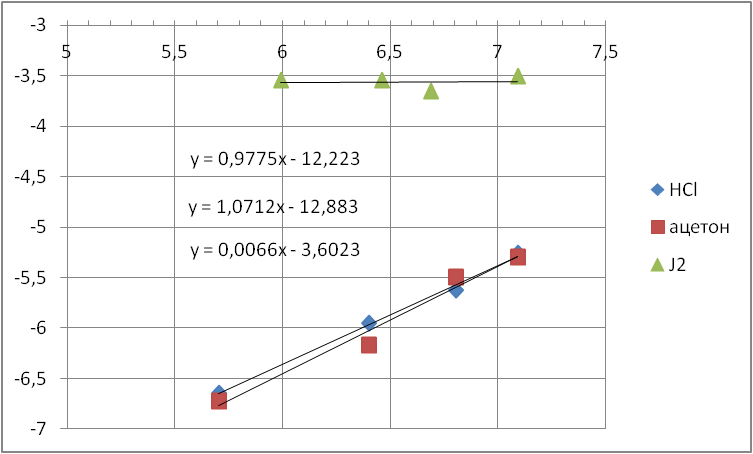
\includegraphics[width=0.8\textwidth]{image002.png}
\end{figure}
Из графика (\ref{lnYlnC}) определяем частные порядки реакции по каждому реагенту:
$$
\begin{array}{llrllll}
	k_{\ce{J2}}&=&0,0066&\pm & 10^{-4}&\approx&0\\
	k_{\ce{HCl}}&=&0,97&\pm &0,06&\approx&1\\
	k_\text{ац}&=&1,07&\pm & 0,16&\approx&1
\end{array}
$$

То есть скорость реакции не зависит от концентрации \ce{J2}.\\

\begin{figure}[h!]
	\centering
	\caption{$y=f(V)$}\label{yC}
	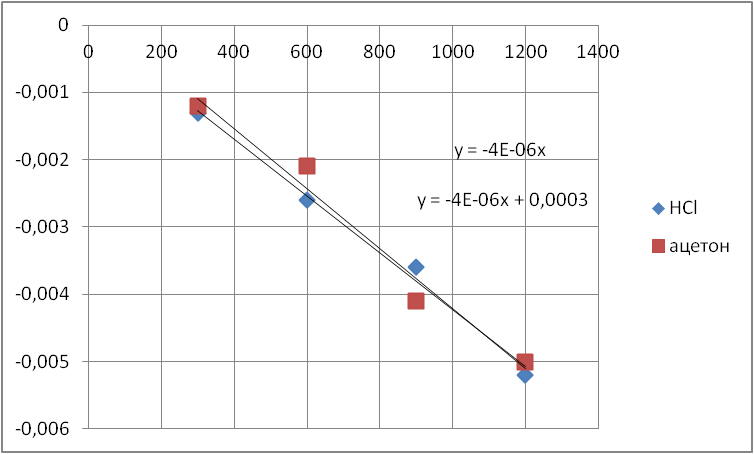
\includegraphics[width=0.8\textwidth]{image003.png}
\end{figure}
Константа скорости $k=(28\pm 3)\cdot 10^{-5} \text{М}^{-1}\text{с}^{-1}$

\newpage
\section{Вывод}

В ходе работы мы подтвердили закон Бера, рассчитали коэффициент экстинкции \\
$\left(\varepsilon_\lambda~=~(340\pm 30)~\textstyle \frac{\text{л}}{\text{моль}\cdot\text{см}}\right)$, определили частные порядки реакции по всем реагентам \\
(0~для~ \ce{J2}, 1 для \ce{HCl} и \ce{C3H6O}) и вычислили константу скорости $\left(k=(28\pm 3)\cdot 10^{-5} \text{М}^{-1}\text{с}^{-1}\right).$
\end{document}